\documentclass[12pt,a4paper]{article}
\usepackage[ansinew]{inputenc} 			% Windows
%\usepackage[latin1]{inputenc} 			% Linux og Mac

\usepackage[T1]{fontenc} 
\usepackage[danish]{babel}				% Dansk ordbog
\usepackage{amsmath, amsfonts, amssymb} % Matematiske pakker
\usepackage{graphicx} 					% Grafiksk pakke
\usepackage{float}						% TIL AT BILLEDER BLIVER HVOR DE ER

\usepackage[left	=3cm,
			right	=2cm,
			top		=2.2cm,
			bottom	=2cm
		]{geometry} 					% Sidejustering

%Mellemrum mellem linjerne
\usepackage{setspace}
\setstretch{1.5} %Afstanden

\usepackage{lastpage}

% Links
\usepackage{hyperref}
\hypersetup{ 
	colorlinks	= true, 	% false: boxed links; true: colored links
    urlcolor	= blue,		% color of external links
    linkcolor	= black, 	% color of page numbers
}

% Figur der st�r vilk�rligt
\usepackage{wrapfig}
%\begin{wrapfigure}{r}{0.6\textwidth}
%	\centering
%	\includegraphics[scale=0.25]{...}
%    \vspace{-20pt}
%    \caption{...}
%  \label{fig:...}
%  \vspace{-10pt}
%\end{wrapfigure}

% Sideops�tning
\usepackage{fancyhdr}					% Header-style
\pagestyle{fancy}
\fancyhf{} % slet alt
\fancyfoot[C]{Side \thepage \text{ af} \pageref{LastPage}} % sidetallet yderst
\lhead[]{\leftmark} % lige side, kapitel titel
\headheight = 35pt
\textheight = 680pt
\footskip 	= 40pt
\rhead{
\begin{picture}(0,0)
\put(-120,0){ 
\includegraphics[scale=0.2]{Diagrammer/Billeder/au-ingenioerhoejskolen_da.jpg}}
\end{picture}}
\renewcommand{\headrulewidth}{0.4pt}
\renewcommand{\footrulewidth}{0.4pt}

\usepackage{enumerate}

\usepackage{subfiles}

%----------------------------------------------------------
% F�lgende er til tabeller
%----------------------------------------------------------
\usepackage{booktabs, cellspace} 		
\addtolength\cellspacetoplimit{10pt}
\addtolength\cellspacebottomlimit{10pt}

%----------------------------------------------------------
% F�lgende er til koder.
% Inds�ttes mellem \begin{lstlisting} og \end{lstlisting}
%----------------------------------------------------------
\usepackage{listings}
\usepackage{color}
\usepackage{textcomp}
\definecolor{listinggray}{gray}{0.9}
\definecolor{lbcolor}{rgb}{0.9,0.9,0.9}
\lstset{
	language		= [Sharp]C,
	keywordstyle	= \bfseries\ttfamily\color[rgb]{0,0,1},
	identifierstyle	= \ttfamily,
	commentstyle	= \color[rgb]{0.133,0.545,0.133},
	stringstyle		= \ttfamily\color[rgb]{0.627,0.126,0.941},
	showstringspaces= false,
	basicstyle		= \small,
	numberstyle		= \footnotesize,
	numbers			= left, % Tal? Udkommenter hvis ikke
	stepnumber		= 1,
	numbersep		= 5pt,
	tabsize			= 2,
	breaklines		= true,
	prebreak 		= \raisebox{0ex}[0ex][0ex]{\ensuremath{\hookleftarrow}},
	breakatwhitespace= false,
	aboveskip		= {1.5\baselineskip},
  	columns			= fixed,
  	upquote			= true,
  	extendedchars	= true,
	lineskip		= 1.5pt,
    xleftmargin		= 17pt,
	framexleftmargin= 17pt,
	framexrightmargin	= 5pt,
	framexbottommargin	= 4pt,
% frame=single,
 	backgroundcolor=\color{lbcolor},
}
\renewcommand*{\lstlistingname}{Kodeudsnit}

\usepackage{caption}
\DeclareCaptionFont{white}{\color{white}}
\DeclareCaptionFormat{listing}{\colorbox[cmyk]{0.43, 0.35, 0.35,0.01}{\parbox{\textwidth}{\hspace{15pt}#1#2#3}}}
\captionsetup[lstlisting]{format=listing,labelfont=white,textfont=white, singlelinecheck=false, margin=0pt, font={bf,footnotesize}}


%----------------------------------------------------------
% F�lgende er tabel over Use Cases - Akt�rer - Forventet 
% 	resultat og checkbox
% Inds�ttes med \begin{testcase} og \end{testcase}
%----------------------------------------------------------
%\usepackage{enumitem,calc}

\newenvironment{testcase}[1]
{
\begin{tabular}{| p{1.2cm} | p{6cm} | p{5.5cm} | l|}\hline
\textbf{TRIN} & \textbf{Aktion / Input} & \textbf{Forventet resultat} & \textbf{CHK} \\
\hline
}
{&\\\hline
\end{tabular}
\\\\}
\newcommand\punkt{&\\\hline} 
\newcommand\Aktion{&}
\newcommand\Forventet{&}

%Grader tegn
\newcommand{\degree}{\ensuremath{^\circ}}

%Bilag kommando
\providecommand{\Bilag}
{ 	\cleardoublepage
	\appendix % Sletter alle kapitelnumre og starter forfra
	\renewcommand{\appendixname}{Bilag} % Fort�ller navnet skal v�re "Bilag"
	\part*{Bilag}
	\addcontentsline{toc}{part}{Bilag}
	\renewcommand{\thesection}{\Roman{section}}
}

% Paragraph instillinger
\renewcommand\paragraph{\@startsection{paragraph}{4}{\z@}%
  {-3.25ex\@plus -1ex \@minus -.2ex}%
  {1.5ex \@plus .2ex}%
  {\normalfont\normalsize\bfseries}}	% Alle indstillinger for dokumentet

%***************************************************
% Det afsnit du arbejder p� skal skrives her
% Inklud�r flere afsnit med komma
% Udkommenter alt du ikke skal bruge med '%'
%
\includeonly{
	Andre_afsnit/Forside,
	Indledning/FormAl,
	Generel_Beskrivelse/Systembeskrivelse,
	Generel_Beskrivelse/Systemets_funktioner,
	Use_Cases/Funktionelle_krav, %Her i ligger Use_Case1
	Use_Cases/Use_Case2,
	Use_Cases/Use_Case3,
	Use_Cases/Use_Case4,
	Use_Cases/Use_Case5,
	Use_Cases/Use_Case6,
	Use_Cases/Use_Case7,
	Eksterne_grEnseflader/Ekstern,
	Andre_afsnit/Kvalitetsfaktorer,
	Andre_afsnit/Designkrav,
	%Andre_afsnit/Ovrigekrav,
	%Andre_afsnit/Delleveringer,
}
%***************************************************

\begin{document}

%---------------------------------------------------
%Herunder skal alle kapitlerne st�.
%
%Hvis der tilf�jes et afsnit, skal det ogs� inkluderes 
%under afsnittet ovenover - adskildt med et komma.
%Tilf�j dit afsnit herunder og udkommenter over over.
%---------------------------------------------------

\newcommand{\HRule}{\rule{\linewidth}{0.8mm}}
\author{TrackABus\\\\Bachelorgr. 13038}
\title{Kravspecifikation}
\date{}

\begin{titlepage}

\begin{center}


% Upper part of the page]    

\textsc{\LARGE TrackABus}\\[1.5cm]

\textsc{\Large Bachelorprojekt}\\[0.5cm]


% Title
\HRule \\[0.4cm]

{ \huge \bfseries Kravspecifikation}\\[0.4cm]
{ \huge \bfseries for}\\[0.4cm] 
{ \huge \bfseries TrackABus}\\[0.4cm]

\HRule \\[1.5cm]

% Author and supervisor
\begin{minipage}{0.4\textwidth}
\begin{flushleft} \large
\emph{Author:}\\
Bachelorgruppe 13038
\end{flushleft}
\end{minipage}
\begin{minipage}{0.4\textwidth}
\begin{flushright} \large
\emph{Supervisor:} \\
Michael Alr�e
\end{flushright}
\end{minipage}

\vfill

% Bottom of the page
{\large \today}

\end{center}

\end{titlepage}

\newpage
\section*{Versionshistorie}


    \begin{tabular}{ | l | l | l | p{10cm} |}
    \hline
    Ver. & Dato & Initialer & Beskrivelse \\ \hline
    0.3 & 06.03.2012 & Gruppe 5 & Skabelon til kravspecifikationen udf�rdiget. \\ \hline
    1.0 & 20.03.2012 & Gruppe 5 & Krav udf�rdiget, mange stadig som brief og casual Use Cases. \\ \hline
    2.0 & 15.04.2012 & Gruppe 5 & Alle Use Cases udf�rdiget som fully dressed. \\ \hline
    3.0 & 17.05.2012 & Gruppe 5 & Dokumentet udf�rdiget til endelig aflevering. \\ \hline
    \end{tabular}

\section*{Godkendelsesformular}
    
    \begin{tabular}{ | l | p{12.4cm} |}
    \hline
    Forfattere 			& Projekt gruppe 5 \\ \hline
    Godkendes af 		& Kunde: Poul Ejnar Rovsing \\& 
    Leverand�r Repr�sentant: Lars Anker Christensen \\ \hline
    Projektnummer 		& 4. Semester projekt \\ \hline
    Dokument-id 		& SBS\_Kravspecifikation \\ \hline
    Antal sider & 31 \\ \hline
    kunde & Poul Ejnar Rovsing \\ \hline
    \end{tabular}  
\\\\
\textbf{Ved underskrivelse af dette dokument accepteres det af begge parter, som v�rende kravene til udviklingen af det �nskede system.}
\\
\\
\textbf{Sted og dato:} \line(1,0){105}
\vspace{1.5cm}
\newpage

\vspace*{1cm}
\begin{tabular}{llp{3cm}ll}
\cline{5-5}
&&&09421 & Lasse Lindsted S�rensen		\\\\\\\cline{5-5}
&&&10063 & Lasse Hansen					\\\\\\\cline{5-5}
&&&10648 & Lars Anker Christensen		\\\\\\\cline{5-5}
&&&10719 & Michael Bojsen-Hansen		\\\\\\\cline{5-5}
&&&10750 & Kasper Vinther Andersen		\\\\\\\cline{5-5}
&&&10770 & Christian Smidt-Jensen		\\\\\\\cline{5-5}
&&&10832 & Christoffer Lousdahl Werge	\\\\\\\cline{5-5}
\cline{1-2} PER & Poul Ejnar Rovsing &&10893 & Rasmus B�kgaard
\end{tabular}

\newpage
\tableofcontents



%1. INDLEDNING
\section{Indledning}

\subsection{Form�l}


Dette dokument har til form�l at opstille de krav, der skal v�re opfyldt, n�r projektet er f�rdiggjort. Dokumentet er blevet udformet af bachelorgruppe 13038, best�ende af Christoffer Lousdahl Werge (studienr. 10832) og Lasse Lindsted S�rensen (studienr. 09421). Disse personer st�r til ansvar for, kravene sat i dette dokument er implementeret ved aflevering. Der er ikke nogen kunde for dette projekt, men vejleder Michael Alr�e agerer kunde i et kvalitetskontrol �jemed. �ndringer i dokumentet efter diskuteres derfor med ham, f�lgende af �ndringerne forklares.   

Kravene er opstillet som en r�kke Use Cases, og de funktionelle krav er derved omdrejningspunktet for dette dokument. De opstillede Use Cases beskriver, hvordan brugeren interragerer med systemet, i en ikke-implementerings specifik forstand.
\\
Det er essentielt at kravene i dette dokument skal f�lges, og ved en endelig accepttest skal alle Use Cases v�re opfyldt til kundens accept.

\subsection{Referencer}
F�lgende dokumenter refereres der til i kravspecifikationen
\begin{itemize}
	\item SBS\_Ide-funktioner.
	\item SBS\_HardwareSpec.
	\item Scorbot-ER 4u, Users Manual -- 100343b ER 4u.
\end{itemize}\
Udover disse dokumenter, er der lavet en accepttest specifikation, der st�r for at verificere at kravene er opfyldt.

\subsection{L�sevejledning}
Det forl�bige navn for projekt er TrackABus, n�r dette navn n�vnes i dokumentet, hentydes der til selve produktet. Der ses herunder en kort beskrivelse af de forskellige afsnit:
\\
\begin{itemize}
\item General Beskrivelse\\
I starten af dokumentet beskrives og illustreres systemet i sin helhed, samt gives der et overblik over systemet funktioner.\\

\item Funktionelle krav\\
Her er alle Use Cases beskrevet fully dressed.\\

\item Eksterne Gr�nseflader\\
Her ses en skitse over hvordan brugergr�nsefladen vil komme til at se ud.

\item Kvalitetsfaktorer og Designkrav\\
Her er beskrevet den kvalitet og den ydelse kunden kan forvente. Derudover kan her ogs� l�ses, hvilke krav der stilles til designer, i forbindelse med implementering\\


\end{itemize}


%2. Generel Beskrivelse
\section{Generel beskrivelse}

\subsection{Systembeskrivelse}

\begin{itemize}

\item Brugersystem \\
Brugersystemet st�r til ansvar for, at brugeren f�r en intuitiv indgang til systemet. Dette system d�kker hele brugeroplevelsen, herunder at kunne v�lge en busrute og se denne p� kortet. Brugersystemet d�kker intet administrativt, og brugeren skal ikke have nogen specielle evner for at bruge denne del af systemet.

\item Administrations system  \\ 
Administrations systemet st�r til ansvar for, at administratoren kan �ndre persisteret data nemt, uden at skulle tilg� databasen direkte. Dette systeme d�kker over en r�kke v�rkt�jer som kan manipulere data for busser og deres ruter. Systemet har ingen p�virkning p� brugersystemet, ud over de �ndringer der sker p� persisteret data.

\item Positionsdata \\
Positionsdata, er infomrationen om bussens placering. Position persisteres direkte, uden om administrations systemet og brugersystemet. Denne del kan simuleres uden tab af funktionalitet.

\item Distribueret persisteret data \\
Persisteret data er kerneelementet i dette projekt. Persisteret data er to-delt og best�r i den globale persisterede data og lokalt persisteret data. Globalt persisteret data vil best� af alt den information brugersystemet og administrations systemet har til f�lles, hvor et eksempel kunne v�re positionsdata. Lokalt persisteret data vil best� af den information brugeren har valgt at gemme lokalt fra brugersystemet, dette vil prim�rt best� af favoriserede busruter. 

\item Lokalt Distribueret data
\end{itemize}

\begin{figure}[u]
\centering
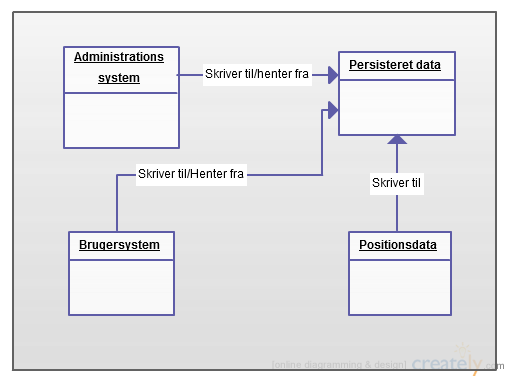
\includegraphics[scale=0.7]{Domainmodel_Billede.jpg}
\caption{Dom�nemodel}
\label{domainmodel}
\end{figure} 

p� figur \ref{domainmodel} gives der et overblik over systemet, hvor enhederne ses i sammenh�ng. De forskellige enheder er beskrevet kort i ovenst�ende afsnit, \emph{2.1 Systembeskrivelse}. Diagramet er lavet med online-v�rk�jet creately.com.

%\subsubsection{Akt�r kontekst-diagram}

\begin{figure}[h]
\centering
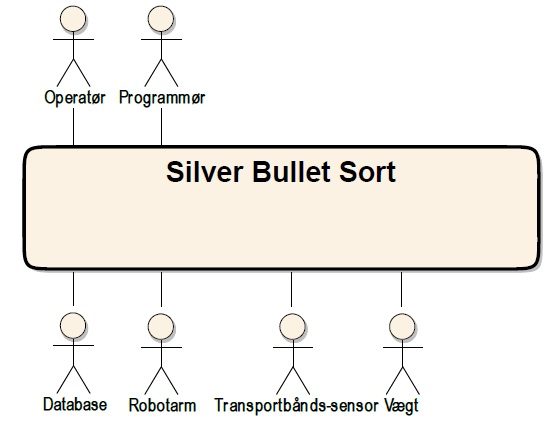
\includegraphics[scale=0.5]{Andet/AktOr-kontekst.jpg}
\caption{Akt�r kontekst-diagram}
\end{figure}

Ovenst�ende figur viser hvilke akt�rer, der interagerer med sorteringssystemet. Videre beskrivelse af disse akt�rer, findes i f�lgende afsnit \emph{2.1.3 Akt�rbeskrivelser}  
\newpage

%\subsubsection{Akt�r beskrivelse}

\underline{\textbf{Prim�re akt�rer:}}\\
\begin{tabular}{lp{10 cm}}

\textbf{Akt�r navn} 				& Operat�r\\
\textbf{Beskrivelse} 				& Denne akt�r starter og stopper systemet. M�let for akt�ren er at f� sorteret klodser, alt efter deres materialetype. \\
\textbf{Antal samtidige akt�rer}	& 1 \\
\\\\
\textbf{Akt�r navn}					&  Programm�r. \\ 
\textbf{Beskrivelse} 				&  Denne akt�rs opgave er at lave brugerdefinerede programmer til systemet.\\ 
\textbf{Antal samtidige akt�rer} 	&  1
\end{tabular}
\\\\
\\\\
\underline{\textbf{Sekund�re akt�rer}}
\\
\begin{tabular}{lp{10 cm}}

\textbf{Akt�r navn} 				& V�gt\\
\textbf{Beskrivelse} 				& Denne akt�r vejer et objekt, s� systemet kan bestemme dets materialetype.  \\
\textbf{Antal samtidige akt�rer}	& 1 \\
\\\\
\textbf{Akt�r navn}					& Transportb�ndssensor \\
\textbf{Beskrivelse}				& Denne akt�r registrerer, hvorn�r et objekt er klar til at blive samlet op af robotten.  \\
\textbf{Antal samtidige akt�rer}	& 1 \\
\\\\
\textbf{Akt�r navn} 				&  Robotarm.\\ 
\textbf{Beskrivelse} 				&  Denne akt�rs opgave er at flytte og m�le forskellige typer klodser.\\ 
\textbf{Antal samtidige akt�rer} 	&  1 \\ 
\\\\
\textbf{Akt�r navn} 				&  Database. \\ 
\textbf{Beskrivelse} 				&  Databasen indeholder logfiler for systemets data for de enkelte klodser, samt informationer om robotten og systemets status. Ligeledes indeholder databasen programmerne, som programm�ren har lavet.\\ 
\textbf{Antal samtidige akt�rer} 	&  1
\end{tabular} 


\subsection{Systemets funktioner}
I det f�lgende punkt er systemets funktioner beskrevet ved Use Case-teknikken. Diagrammet nedenfor giver overblik over systemets funktioner.

\subsubsection{Use Case diagram}

\begin{figure}[h]
\centering
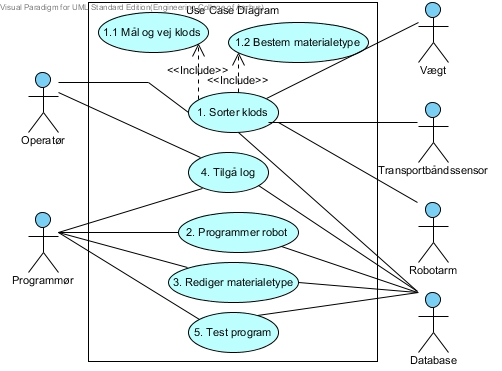
\includegraphics[scale=0.6]{Use_Cases/Diagrammer/Use_Case_Diagram.jpg} 
\caption{Use Case diagram}
\end{figure}

Hovedfunktionen i systemet er, at lade en bruger finde ud, hvor en given bus befinder sig p� et rute, ud fra et valgt stoppested. Brugeren vil v�lge en rute, hvorefter han vil kunne se alle busser p� den valgte rute. Herefter vil han kunne v�lge et stoppested, og herefter vil kun den n�rmeste (og muligvis n�stn�rmeste, se Use Case 3, untagelse 5 REFERENCE THIS) vises p� kortet. Udover dette vil en estimeret tid for ankomst af den n�rmeste bus til stoppestedet vises.
\\ 
En administrator kan �ndre ruteplaner, busser og busnumre i et seperat system.

\\\\
De forskellige Use Cases er detaljeret beskrevet senere i dokumentet, i afsnittet \textit{3 Funktionelle krav - Use Cases}
\subsection{Systemets begr�nsninger}
I produktopl�gget er et kamera beskrevet. I det endelige produkt er dette erstattet af en optisk sensor, som indg�r i styringen af transportb�ndet. Dette er foretaget efter aftale med kunde.\\
Den manuelle pendant er desuden fjernet, og i stedet kan robotten programmeres via et user interface p� en PC.

\subsection{Brugerprofil}
Det forventes at den administrative del, kun opereres af en person, som er orienteret i funktionerne for denne del af systemt.
\begin{itemize}

\item Brugeren \\
Brugeren er en prim�r akt�r af systemet. Det er ikke essentielt at denne person har nogen forst�else for, hvad der foreg�r bag systemet. Det eneste krav der stilles til brugeren er, at personen skal tilg� systemet fra en android platform.
\item Administrator \\
Administratoren er en prim�r akt�r af systmet. Det er ikke essentielt at denne person har forst�else for, hvordan en database virker. Det er dog vigtigt at personen er tr�net i at bruge denne del af systemet, og har en forst�else for, hvad de �ndringerne der foretages, g�r. Da administratoren bliver pr�senteret for et r�kke v�rkt�j, skal personen ikke n�dvendigvis have specielle kompetencer.

\end{itemize}


\subsection{Krav til udviklingsforl�bet}
Selvom der ikke blev vedlagt mange obligatoriske krav til dette projekt, er der i gruppen blevet fastlagt nogle udviklingsm�ssige rammer, som vil blive fulgt:

\subsubsection{Obligatoriske udviklingsv�rkt�jer}
Programmeringssproget skal i dette projekt v�re C\#, hvor der skal g�res brug af WPF til det grafiske interface samt .NET 4.0 frameworket. Til persistente data skal der g�res brug af SQL databaser, herunder logning og lagering af data fra klodserne. Undervejs i projektet udarbejdes to store dokumenter, en processrapport og et designdokument. \\

\subsubsection{Gruppedefinerede udviklingsv�rkt�jer}
Til selve udviklingen er der blevet valgt at f�lge v�sentlige principper fra Scrum frameworket. Der blev gjort brug af dette i tredje semesterprojektet, hvor det blev set som ganske brugbart. Herunder blev der ogs� gjort brug af nogle af Extreme Programming-principperne. \\ 




\subsection{Foruds�tninger}
Det forventes at der kan skabes en l�bende kommunikation med kunden (Michael Alr�e, ma@iha.dk). Hertil vil der l�bende blive holdt m�der, hvor �ndringer diskuteres.


\subsection{Systemets begr�nsninger}
I produktopl�gget er et kamera beskrevet. I det endelige produkt er dette erstattet af en optisk sensor, som indg�r i styringen af transportb�ndet. Dette er foretaget efter aftale med kunde.\\
Den manuelle pendant er desuden fjernet, og i stedet kan robotten programmeres via et user interface p� en PC.

\subsection{Brugerprofil}
Det forventes at den administrative del, kun opereres af en person, som er orienteret i funktionerne for denne del af systemt.
\begin{itemize}

\item Brugeren \\
Brugeren er en prim�r akt�r af systemet. Det er ikke essentielt at denne person har nogen forst�else for, hvad der foreg�r bag systemet. Det eneste krav der stilles til brugeren er, at personen skal tilg� systemet fra en android platform.
\item Administrator \\
Administratoren er en prim�r akt�r af systmet. Det er ikke essentielt at denne person har forst�else for, hvordan en database virker. Det er dog vigtigt at personen er tr�net i at bruge denne del af systemet, og har en forst�else for, hvad de �ndringerne der foretages, g�r. Da administratoren bliver pr�senteret for et r�kke v�rkt�j, skal personen ikke n�dvendigvis have specielle kompetencer.

\end{itemize}


\subsection{Krav til udviklingsforl�bet}
Selvom der ikke blev vedlagt mange obligatoriske krav til dette projekt, er der i gruppen blevet fastlagt nogle udviklingsm�ssige rammer, som vil blive fulgt:

\subsubsection{Obligatoriske udviklingsv�rkt�jer}
Programmeringssproget skal i dette projekt v�re C\#, hvor der skal g�res brug af WPF til det grafiske interface samt .NET 4.0 frameworket. Til persistente data skal der g�res brug af SQL databaser, herunder logning og lagering af data fra klodserne. Undervejs i projektet udarbejdes to store dokumenter, en processrapport og et designdokument. \\

\subsubsection{Gruppedefinerede udviklingsv�rkt�jer}
Til selve udviklingen er der blevet valgt at f�lge v�sentlige principper fra Scrum frameworket. Der blev gjort brug af dette i tredje semesterprojektet, hvor det blev set som ganske brugbart. Herunder blev der ogs� gjort brug af nogle af Extreme Programming-principperne. \\ 




\subsection{Foruds�tninger}
Det forventes at der kan skabes en l�bende kommunikation med kunden (Michael Alr�e, ma@iha.dk). Hertil vil der l�bende blive holdt m�der, hvor �ndringer diskuteres.


%3. Use Cases
\section{Funktionelle krav - Use Cases}
\subsection{Use Case 1: Vis busruter}
\textbf{M�l:}
\\
M�let med denne Use Case er at f� vist alle distribuerede persisterede busruter. 
\\
\\
\textbf{Initiering:}
\\
Brugeren tilkendegiver over for systemet, at han �nsker at f� vist alle distribuerede persisterede busruter. 
\\
\\
\textbf{Akt�rer og interessenter:}
\\
Prim�re akt�rer:
\begin{itemize}
\item Bruger.
\end{itemize}
\textbf{Antal samtidige forekomster:}
\\
En samtidig forekomst.
\\
\\
\textbf{Ikke funktionelle krav:} \\
Ingen\\

\noindent
\textbf{Startbetingelser:}
\\
Programmet er startet op, og brugeren st�r ved startsk�rmen.(Se figur \ref{fig:MainScreen})
\\
\\
\textbf{Slutresultat ved succes:}
\\
Brugeren f�r vist en liste over alle distribuerede persisterede busruter.(Se figur \ref{fig:RouteListScreen})
\\
\\
\textbf{Slutresultat ved undtagelser:}
\\
Brugeren f�r vist startsk�rmen.
\\
\\
\textbf{Normalforl�b A:}

\begin{enumerate}
\item Systemet tilg�r distribueret persisteret data, og henter busruterne.
\item Systemet pr�senterer brugeren overfor listen af busruter.
\end{enumerate}
\textbf{Undtagelser:}
\begin{enumerate}[\text{Undtagelse} A:] 
\item Persisteret data kan ikke tilg�s.

	\begin{enumerate}[1.]
	\item Systemet viser en fejlmeddelelse til brugeren, der beskriver, at det ikke er muligt at indl�se busruterne.
	\item Systemet returnerer til startsk�rmen.
	\end{enumerate}
\end{enumerate}

\begin{enumerate}[\text{Undtagelse} B:] 
\item Brugeren annullerer indl�sningen. 
	\begin{enumerate}[1.]
	\item Systemet annullerer indl�sningen af data.
	\item Systemet returnerer til startsk�rmen.
	\end{enumerate}
\end{enumerate}

\begin{enumerate}[\text{Undtagelse} C:] 
\item Systemet g�r i dvale, under indl�sningen. 
	\begin{enumerate}[1.]
	\item Systemet indl�ser busruterne f�rdig i baggrunden.
	\end{enumerate}
\end{enumerate}
\subsection{Use Case 2: Programmer robot}
\textbf{M�l:}
\\
M�let med denne Use Case er at omprogrammere robotten til at tjene et nyt form�l eller udf�re samme opgave p� en ny m�de samt at anvende selve programmet.
\\\\
\textbf{Initiering:}\\
Programm�ren tilkendegiver over for systemet, at han �nsker at �ndre i programmer eller anvende et program.
\\\\
\textbf{Akt�rer og interessenter:}
\\
Prim�re akt�rer:
	\begin{itemize}
	\item Programm�r.
	\end{itemize}
Sekund�re akt�rer:
	\begin{itemize}
	\item Ingen.
	\end{itemize}
\textbf{Antal samtidige forekomster:}
\\
En samtidig forekomst.
\\\\
\textbf{Ikke funktionelle krav:}
	\begin{itemize}
	\item Ingen.
	\end{itemize}
\textbf{Referencer:}\\
SBS\_Ide-funktioner.pdf.\footnote{Dokumentet beskriver de funktioner programm�ren kan bruge til at programmere robotten}
\\\\
\textbf{Startbetingelser:}
\\
Brugeren skal v�re logget ind som 'programm�r'.\footnote{G�lder ikke for normalforl�b 4, da operat�ren ogs� kan anvende et program.}
\\\\
\textbf{Slutresultat ved succes:}
\\
Programm�ren har f�rdiggjort eller �ndret i et program, og programmet/�ndringerne er blevet gemt. Hvis et program �nskes anvendt, er dette blevet anvendt.
\\\\
\textbf{Slutresultat ved undtagelser:}
\\
Programmet eller �ndringerne er ikke blevet gemt og programmet er ikke blevet anvendt. 
\\\\
\textbf{Normalforl�b 1 - Opret nyt program:}
	
	\begin{enumerate}
	\item Programm�ren tilkender overfor systemet, at han vil redigere i programmer.
	\item Systemet �bner faciliteter for at kunne �ndre styringen til robotten.
	\item Programm�ren laver den nye styring.
	\item Programm�ren tilkendegiver over for systemet, at programmet skal gemmes.
	\item Systemet gemmer programmet.
	\end{enumerate}
\textbf{Undtagelser 1 - Opret nyt program:}

	\begin{enumerate}[\text{Undtagelse 3} a:]

	\item Programm�ren afslutter program uden at gemme.
		
		\begin{enumerate}
		\item Systemet sp�rg programm�ren, om han er sikker p�, at programmet skal lukkes uden at gemmes.
		\end{enumerate}
	\end{enumerate}
	
	\begin{enumerate}[\text{Undtagelse 4} a:]
	\item Programm�ren har ikke navngivet programmet.
		
		\begin{enumerate}
		\item Systemet tilkendegiver over for programm�ren at programmet skal gemmes med et navn.
		\item Programm�ren giver navn for program.
		\end{enumerate}
	
	\end{enumerate}
\textbf{Normalforl�b 2 - Rediger gammelt program:}
	
	\begin{enumerate}
	\item Programm�ren tilkender overfor systemet, at han vil redigere i programmer.
	\item Systemet lister gamle programmer, der er tilg�ngelige.
	\item Programm�ren tilkendegiver, hvilket program fra listen denne �nsker at redigere.
	\item Systemet �bner faciliteter for at kunne �ndre styringen til robotten.
	\item Programm�ren redigerer den gamle styring.
	\item Programm�ren tilkendegiver over for systemet, at denne skal gemme programmet.
	\item Systemet gemmer programmet.
	\end{enumerate}	
\textbf{Undtagelser 2 - Rediger gammelt program:}
	
	\begin{enumerate}[\text{Undtagelse 2} a:]
	\item Der er ingen gamle programmer tilg�ngelige.
		
		\begin{enumerate}
		\item Der fremkommer ingen gamle programmer.
		\end{enumerate}
	\end{enumerate}
	
		\begin{enumerate}[\text{Undtagelse 3} a:]
	\item Programm�ren v�lger standardprogrammet.
		
		\begin{enumerate}
		\item Programm�ren modtager en besked om, at det ikke er muligt at redigere i standardprogrammet. 
		\end{enumerate}
	
	\end{enumerate}
	
	\begin{enumerate}[\text{Undtagelse 7} a:]
	\item Programm�ren afslutter program uden at gemme.		
		\begin{enumerate}
		\item Systemet giver programm�ren en meddelelse, om han �nsker at afslutte uden at gemme.
		\end{enumerate}
	\end{enumerate}
\textbf{Normalforl�b 3 - Slet program:}
	\begin{enumerate}
	\item Programm�ren tilkender overfor systemet, at han vil redigere i programmer.
	\item Systemet lister gamle programmer, der er tilg�ngelige.
	\item Programm�ren tilkendegiver overfor systemet, hvilket program der �nskes slettet.
	\item Systemet sp�rger programm�ren, om handlingen �nskes udf�rt.
	\item Programm�ren tilkendegiver overfor systemet, at dette �nskes.
	\item Systemet sletter programmet.
	\end{enumerate}
\textbf{Undtagelser 3 - Slet program:}
	\begin{enumerate}[\text{Undtagelse 2} a:]
	\item Der er ingen gamle programmer tilg�ngelige.	
		\begin{enumerate}
		\item Der fremkommer ingen gamle programmer.
		\end{enumerate}
	\end{enumerate}
	\begin{enumerate}[\text{ Undtagelse 3} a:] 
	\item Programm�ren har valgt standardprogrammet.
		
		\begin{enumerate}
		\item Systemet giver en besked om, at det ikke er muligt at slette standardprogrammet.
		\end{enumerate}
	
	\end{enumerate}	
	

	\begin{enumerate}[\text{ Undtagelse 5} a:] 
	\item Programm�ren tilkendegiver overfor systemet, at programmet ikke �nskes slettet alligevel.	
		\begin{enumerate}
		\item Systemet sletter ikke programmet.
		\end{enumerate}
	\end{enumerate}
\textbf{Normalforl�b 4 - Anvend program:}	
	\begin{enumerate}
	\item Programm�ren tilkendegiver over for systemet, at han vil anvende et program. 
	\item Systemet lister programmer, der er tilg�ngelige.
	\item Programm�ren tilkendegiver over for systemet, hvilket program fra listen denne �nsker at anvende.
	\item Det valgte program anvendes. 
	\end{enumerate}
\textbf{Undtagelser 4 - Indl�s gammelt program:}	
	\begin{enumerate}[\text{Undtagelse 2} a:]
	\item Der er ingen gamle programmer tilg�ngelige.
		
		\begin{enumerate}
		\item Programm�ren kan kun v�lge standardprogrammet.
		\end{enumerate}
	
	\end{enumerate}








\subsection{Use Case 3: Vis tid for n�rmeste bus, til valgt stoppested.}
\textbf{M�l:}
\\
M�let med denne Use Case er at f� vist tid til ankomst, for den bus der er t�ttest p� et valgt busstoppested.
\\
\\
\textbf{Initiering:}
\\
P� kortet skabt af normalforl�bet i Use Case 2, v�lger brugeren et stoppested.
\\
\\
\textbf{Akt�rer og interessenter:}
\\
Prim�re akt�rer:
	\begin{itemize}
	\item Bruger
	\end{itemize}
\textbf{Antal samtidige forekomster:}
\\
En samtidig forekomst.
\\
\\
\textbf{Ikke funktionelle krav:}
	\begin{itemize}
	\item Opdatering af tid sker hver andet sekund, med en max. afvigelse p� 0.5 sekunder.
	\item Tid vil opskrives p� formen "tt:mm:ss", hvor tt er timer, mm er minutter og ss er sekunder
	\item Ved ingen k�rende busser imod valgt stoppested, vil tid vises som "nn:nn:nn"
	\end{itemize}
\textbf{Startbetingelser:}
\\

Normalforl�b for Use Case 2 er blevet gennemf�rt.
\\
\\
\textbf{Slutresultat ved succes:}
\\
Brugeren bliver pr�senteret for et kort, med indtegnet busrute samt tid til ankomst for n�rmeste bus til valgt stoppested.
\\
\textbf{Slutresultat ved undtagelser:}
\\
Brugeren bliver pr�senteret for et kort, med indtegnet busrute.
\\
\\
\textbf{Normalforl�b:}
\begin{enumerate}
\item Brugeren bliver vist tiden indtil bussen ankommer til det valgte busstoppested, samt information om busstoppestedet.
\end{enumerate}

\begin{enumerate}[\text{Undtagelse} 1:]
	\item Positions data kan ikke tilg�s.
	\begin{enumerate}[A]
		\item Systemet viser en fejlmeddelelse til brugeren, der beskriver, at det ikke er muligt at tilg� positionsdata busserne.
		\item Brugeren vil blive vist kortet, hvor busserne ses p� deres senest hentede position. Bussens position opdateres ikke l�ngere.
	\end{enumerate}
\end{enumerate}		
\begin{enumerate}[\text{Undtagelse} 2:]
	\item Positions data for n�rmeste bus kan igen tilg�s.
	\begin{enumerate}[1.]
		\item Systemet forts�tter i normalforl�bet. Bussernes position holdes igen opdateret
		\item Systemet fjerner fejl-meddelelsen igen.
	\end{enumerate}
\end{enumerate}
\begin{enumerate}[\text{Undtagelse} 3:]
	\item Hentningen af data annulleres.
	\begin{enumerate}[1.]
		\item Systemet stopper med at hente bussernes positions data.
		\item Systemet returnerer til listen over busruter.
	\end{enumerate}
\end{enumerate}
\begin{enumerate}[\text{Undtagelse} 4:]
	\item Systemet g�r i dvale, under hentning af data.
	\begin{enumerate}[1.]
		\item Systemet henter data f�rdige, og v�rdier opdateres.
		\item Systemet g�r i dvale. bussernes position vil ikke l�ngere holdes opdateret.
	\end{enumerate}
\end{enumerate}
\include{Use_Cases/Use_Case4}
\subsection{Use Case 5: Test program}
\textbf{M�l:}
\\
M�let med denne Use Case er at teste er et f�rdigt program eller en programsekvens via en simulering af robotten.
Det giver programm�ren mulighed for at teste sit program uden brug af robotten.
\\
\\
\textbf{Initiering:}
\\
Programm�ren starter tilkendegiver overfor systemet, at han vil starte en simulering.
\\
\\
\textbf{Akt�rer og interessenter:}
\\
Prim�re akt�rer:
\begin{itemize}
\item Programm�ren.
\end{itemize}
Sekund�re akt�rer:
\begin{itemize}
\item Ingen.
\end{itemize}
\textbf{Antal samtidige forekomster:}
\\
En samtidig forekomst.
\\
\\
\textbf{Ikke funktionelle krav:}
\begin{itemize}
\item Simuleringsbeskeder udskrives med et tidspunkt for begivenheden sammen med informationer om selve handlingen.
\end{itemize}
\textbf{Referencer:}
\\
Ingen.
\\\\
\textbf{Startbetingelser:}
\\
Det foruds�ttes, at brugeren er logget ind som programm�r.
\\
\\
\textbf{Slutresultat ved succes:}
\\
Programm�ren f�r fuldendt en testsimulering af programmet.
\\
\\
\textbf{Slutresultat ved undtagelser:}
\\
Programm�ren f�r ikke fuldendt en testsimulering af programmet
\\
\\
\textbf{Normalforl�b:}
\begin{enumerate}
\item Programm�ren tilkendegiver over for systemet at vedkommende �nsker en simulering.
\item Systemet indl�ser tilg�ngelige programmer.
\item Programm�ren v�lger en af programmerne.
\item Programm�ren starter simuleringen af programmet.
\item Alle systemets informationer fra programmet gemmes i en simuleringslogfil.
\item Simulationen afsluttes.
\end{enumerate}

\textbf{Undtagelser:}
\begin{enumerate}[\text{Undtagelse *} a:] 
\item Programm�ren trykker p� stop.
	\begin{enumerate}[1.]
	\item Simuleringen stoppes.
	\end{enumerate}
\end{enumerate}



\include{Use_Cases/Use_Case6}
\subsection{Use Case 7: Tilf�j/Fjern/�ndre busruteplan}
\textbf{M�l:}
\\
M�let med denne Use Case er, at kunne tilf�je, fjerne eller �ndre en busruteplan. Med tilf�jelse menes der, at en hel ny ruteplan bliver persisteret. Med fjernelse menes der, at en allerede persisteret rute bliver fjernet. Med �ndring menes der, at der �ndres i en allerede persisteret ruteplan.
\\
\\
\textbf{Initiering:}
\\
Administratoren tilkendegiver over for systemet at han �nsker at lave �ndringer i ruteplanen for en bus. Herefter bliver han stillet overfor valget, om han �nsker at tilf�je en ny ruteplan, fjerne en allerede eksisterende ruteplan, eller �ndre den eksisterende ruteplan.
\\
\\
\textbf{Akt�rer og interessenter:}
\\
Prim�re akt�rer:
\begin{itemize}
\item Administrator.
\end{itemize}
\textbf{Antal samtidige forekomster:}
\\
En samtidig forekomst.
\\
\\
\textbf{Ikke funktionelle krav:}
\begin{itemize}
\item Kommer Senere
\end{itemize}
\textbf{Startbetingelser:}
\\
Man skal have administrator rettigheder, for at kunne tilg� denne del af systemet.
\\
\\
\textbf{Slutresultat ved succes:}
\\
En ny busrute vil v�re tilf�jet til listen over ruter og persisteret.\\
En allerede persisteret busrute vil blive fjernet fra persisteringen og slettet.\\
En allerede persisteret busrute vil blive �ndret, og �ndringerne p� ruten vil blive persisteret.
\\
\\
\textbf{Slutresultat ved undtagelser:}
\\
Den valgte busrute vil ikke blive opdateret. Hvis administratoren har lavet �ndringer og trykker annuller eller lukker systemet, vil en meddelelse blive vist. Denne meddelelse sp�rger om der �nskes at gemmes f�r lukning.
\\
\\
\textbf{Normalforl�b A: Tilf�jelse af busrute}
	\begin{enumerate}
	\item Administrator tilkendegiver overfor systemet, at der �nskes at tilf�jes en busrute.
	\item Et v�rkt�j bliver pr�senteret, hvor et tomt kort kan ses. Her kan der tilf�jes en ny rute, med veje og busstoppesteder.
	\item Administratoren skaber en rute.
	\item Der tilkendegives overfor systemet, at ruten skal gemmes.
	\item Den tilf�jede rute persisteres.
	\end{enumerate}
	\textbf{Normalforl�b B: Fjernelse af busrute}
	\begin{enumerate}
	\item Administrator tilkendegiver overfor systemet, at der �nskes at fjerne en allerede persisteret rute.
	\item Det tilkendegives overfor systemet, at fjernelsen af ruten skal gemmes.
	\item Den valgte rute fjernes fra persisteringen.
	\end{enumerate}
	\textbf{Normalforl�b C: �ndring af busrute}
	\begin{enumerate}
	\item Administrator tilkendegiver over for systemet, at der �nskers at �ndre en given busrute.
	\item Et v�rkt�j bliver pr�senteret, med den valgte rute indtegnet. Her kan der tilf�jes eller fjernes veje og busstoppesteder.
	\item Administratoren �ndrer ruten.
	\item Der tilkendegives over for systemet, at �ndringer skal gemmes.
	\item Den �ndrede rute persisteres.
	\end{enumerate}
\textbf{Undtagelser}
	\begin{enumerate}[\text{Undtagelse 1}]

	\item Administratoren annullerer �ndringsprocessen, f�r tilf�jelser, fjernelser eller �ndringer er foretaget.
		
		\begin{enumerate}[A]
		\item Der returneres til administrations-hovedsk�rmen.
		\end{enumerate}
	\end{enumerate}
		\begin{enumerate}[\text{Undtagelse 2}]

	\item Administratoren annullerer �ndringsprocessen, efter tilf�jelser, fjernelser eller �ndringer er foretaget.
		
		\begin{enumerate}[A]
		\item Administratoren bliver pr�senteret for en meddelelse , hvori der bliver spurgt, om der vil gemmes eller ej.
		\begin{enumerate}[1]
		\item Hvis der ikke �nskes at gemmes, returneres der til administrations-hovedsk�rmen.
		\item Hvis der �nskes at gemmes, bliver �ndringerne persisteret. Herefter returneres der til administrations-hovedsk�rmen.
		\end{enumerate}
		\end{enumerate}
	\end{enumerate}
		\begin{enumerate}[\text{Undtagelse 3}]

	\item Det er ikke muligt at persistere data.
		
		\begin{enumerate}[A]
		\item Administratoren bliver pr�senteret for en fejlmeddelelse, som informerer om, at det ikke er muligt at persistere �ndret data.
		\item Der returneres til det sted administratoren arbejdede, hvor de �ndringer han har foretaget, stadig er tilstede.
		\end{enumerate}
	\end{enumerate}
	




%4. EKSTERNE GR�NSEFLADER	
\section{Eksterne gr�nseflader}
\subsection{Brugergr�nseflade}
Der er blevet udformet en skitse over brugergr�nsefladen, s� kunden kan f� en id� om, hvordan det grafiske vil komme til at se ud. Det er vigtigt at understrege, at det er en \underline{skitse}, og at den endelige brugergr�nseflade ikke n�dvendigvis vil ligne denne fuldst�ndigt:\\

\begin{figure}[h]
\centering
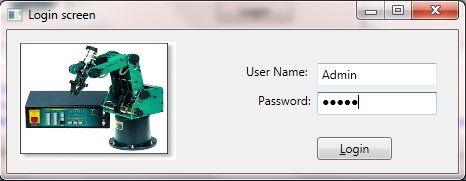
\includegraphics[scale=1]{Eksterne_grEnseflader/GUI/LoginScreen.JPG}
\caption{Loginvindue}
\end{figure}

\begin{figure}[h]
\centering
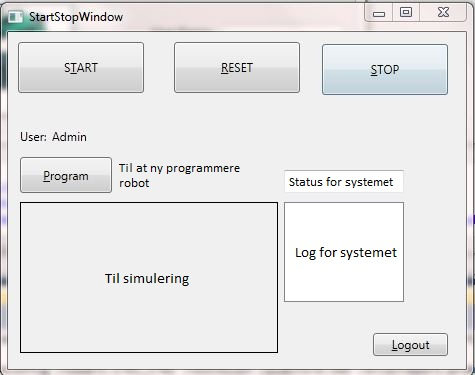
\includegraphics[scale=1]{Eksterne_grEnseflader/GUI/StartStopWindowSomAdmin.JPG}
\caption{K�rselsvindue}
\end{figure}

\begin{figure}[h]
\centering
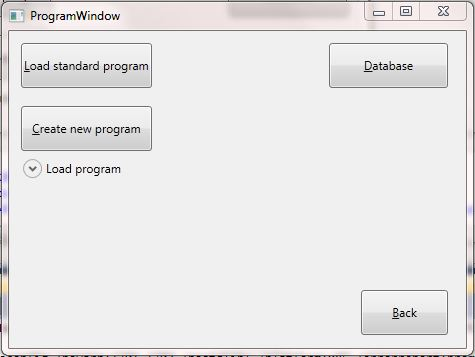
\includegraphics[scale=1]{Eksterne_grEnseflader/GUI/ProgrammingWindow.JPG}
\caption{Programmeringsvindue}
\end{figure}
%\newpage
\subsection{Hardware gr�nseflader}
Hardware-specifikationerne kan ses i dokumentet "Hardwarespec". I dette dokument er der beskrevet hvordan de forskellige hardware-enheder er forbundet og gr�nsefladen mellem dem. 

%5. Andre afsnit
\section{Kvalitetsfaktorer}

\begin{itemize}
\item \textbf{Brugervenlighed:} \\
Der vil blive sat stort focus p� at g�re brugersystemet brugervenligt og intuitivt, da systemet skal kunne bruges uden nogle vejledning eller anden form for introduktion.
\item \textbf{P�lidelighed} \\
Brugersystemet skal v�re p�lideligt, da placeringen af busserne, samt tiden til ankomst ved valgt stoppested skal v�re pr�cise. Hvis dette ikke er pr�cis vil det g� imod form�let med systemet.
\item \textbf{Effektivitet} \\
Systemet skal v�re hurtigt, s� en bruger ikke skal vente i l�ngere tid p� at f� det �nskede information.
\end{itemize}
\section{Designkrav}
\begin{itemize}
\item Systemet implementeres i det objektorienteret programmeringssprog, C\#.
\item Funktionsstrukturen i IDE'en skal minde om den, der er i det udleverede Scorbase-program.
\item Robotten skal programmeres via det udleverede bibliotek USBC.dll.

\end{itemize}


%\section{�vrige krav}
\end{document}
